\usetikzlibrary{shapes.gates.logic.US}
\def\itemlabel{(a)}
\def\NOT#1{\overline{#1}}
\def\nota{\NOT{A}}
\def\notb{\NOT{B}}
\def\notc{\NOT{C}}
\def\notx{\NOT{x}}


\question{5} Analise os circuitos a seguir e descreva-os utilizando 
a álgebra Booleana:\\

Circuito 1

\begin{figure}[h]
\begin{center}
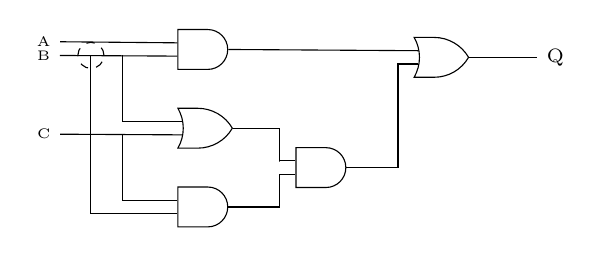
\begin{tikzpicture}
  \node[name=a,draw, and gate US]  at (0,3.25) {};
  \node[name=A] at (-2,3.35) {\tiny A};
  \draw[] (A) -- (a.input 1);

  \node[name=b,draw, or gate US]  at (0,2.25) {};
  \node[name=B] at (-2,3.175) {\tiny B};
  \draw[] (B) -- (a.input 2);
  \node[name=C] at (-2,2.175) {\tiny C};
  \draw[] (C) -- (b.input 2);
  \draw (b.input 1) -| (-1,3.175) node[] {};

  \node[name=c,draw, and gate US] at (0,1.25) {};
  \draw (c.input 1) -| (-1,2.175) {};
  \draw (c.input 2) -| (-1.4,3.175) node[circle,draw,dashed] (1pt) {};


  \node[name=d,draw, or gate US] at (3,3.15) {};
  \node[name=C] at (4.5,3.15) {\scriptsize Q};
  \draw[] (d.output) -- (C);

  \node[name=e,draw, and gate US] at (1.5,1.75) {};
  \draw[] (a.output) -- (d.input 1);
  \draw[] (b.output) -| (1,1.825) |- (e.input 1);
  \draw[] (c.output) -| (1,1.25) |- (e.input 2);
  \draw[] (e.output) -| (2.5,3) |- (d.input 2);

  \end{tikzpicture}
\end{center}
\caption{Circuito lógico combinacional 1}
\label{fig:fourgates}
\end{figure}

% Resposta: $AB+BC(B+C)$ 


Circuito 2
\begin{figure}[ht]
\begin{center}
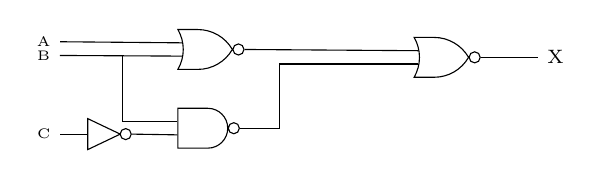
\begin{tikzpicture}
  \node[name=a,draw, nor gate US]  at (0,3.25) {};
  \node[name=A] at (-2,3.35) {\tiny A};
  \draw[] (A) -- (a.input 1);

  \node[name=b,draw, nand gate US]  at (0,2.25) {};
  \node[name=B] at (-2,3.175) {\tiny B};
  \draw[] (B) -- (a.input 2);
  \node[name=C] at (-2,2.175) {\tiny C};
  \node[name=n,draw, not gate US]  at (-1.3,2.175) {};
  \draw (C) -- (n.input);
  \draw (n.output) -- (b.input 2);
  \draw (b.input 1) -| (-1,3.175) node[circle] {};


  \node[name=c,draw, nor gate US] at (3,3.15) {};
  \node[name=X] at (4.5,3.15) {\scriptsize X};
  \draw (a.output) -- (c.input 1);
  \draw (c.output) -- (X);
  \draw (b.output) -| (1,2.75) |- (c.input 2) {};

  \end{tikzpicture}
\end{center}
\caption{Circuito lógico combinacional 2.}
\label{fig:circ}
\end{figure}\\

% Resposta $\NOT{\NOT{(A+B)}+\NOT{B\NOT{C}}}$


\question{2,0}~Realize as seguintes divisões binárias, mostrando os
cálculos intermediários:

\begin{enumerate}[(a)]
\item $1100\div100$
\item $111111\div1001$
\end{enumerate}

\question{2,0}~Faça a tabela-verdade para o circuito da
Figura~\ref{fig:circ}.

\question{4,0} Simplifique as expressões Booleanas a seguir:

\begin{enumerate}[(a)]
\item $ABC+AB\NOT{C}+A\NOT{B}C+ABC$

% Resposta: $A(B+C)$

% Resolução:
% $$ABC+AB\notc+A\notb C+ABC = AB(C+\notc)+AC(B+\notb)$$
% ({\scriptsize $x+\notx=1$)}
% $$AB+AC=$$
% $$A(B+C)$$

\item $(\NOT{A}+B)(A+B+C)\NOT{C}$


%  Resposta: $B\NOT{C}$ 
%  Resolução:

% $$(\nota+B)(A+B+C)\notc = (A\nota+\nota{}B+\nota{}C+AB+BB+BC)\notc=$$
% $$A\nota\notc+\nota B\notc+\nota C\notc+AB\notc+BB\notc+BC\notc=$$
% ({\scriptsize $\notx{}x=0$ e $xx=x$})
% $$\nota B\notc+AB\notc+B\notc = B\notc(A+\nota+1)=$$
% ({\scriptsize $x+\notx=1$})
% $$B\notc$$

\item $(\NOT{A+\NOT{B}C})+(\NOT{A+B})$

\item $\NOT{ABC}(\NOT{A+B+C})$

\end{enumerate}

\newpage\input ../_slides/teoremas


\question{3} Para cada uma das expressões booleanas a seguir,
desenhe o circuito lógico correspondente usando as portas
{\tt AND}, {\tt OR} e {\tt NOT}.

\begin{enumerate}[(a)]
\item $x=AB(C+\NOT{B})$
\item $y=\NOT{A+B\NOT{C}}$
\end{enumerate}


\question{2} Para quais entradas (valores) de $A$, $B$, $C$,
respectivamente, do circuito da Figura~\ref{fig:circ}, a saída $X$
será $1$? (Dica: Use a tabela-verdade para a análise.)

% Resolução:  0,1,0 

% \bigskip
% \begin{center}
% \begin{tabular}{|c|c|c|c|c|c|c|}
% $A$ & $B$ & $C$ &$y=\NOT{A+B}$ &$\notc$ & $z=\NOT{B\notc}$
% &$x=\NOT{y+z}$ \\\hline
% 0 & 0 & 0 & 1 & 1 & 1 & 0\\
% 0 & 0 & 1 & 1 & 0 & 1 & 0\\
% 0 & 1 & 1 & 0 & 0 & 1 & 0\\
% 1 & 1 & 1 & 0 & 0 & 1 & 0\\\hline
% 1 & 1 & 0 & 0 & 1 & 0 & 1\\\hline
% 1 & 0 & 0 & 0 & 1 & 1 & 0\\
% 1 & 0 & 1 & 0 & 0 & 1 & 0\\\hline
% \bf 0 & \bf 1 & \bf 0 &\bf 0 &\bf 1 &\bf 0 &\bf 1\\\hline

% \end{tabular}
% \end{center}


